\section{Motivation} \label{sec:motivation}

The fingerprint-based ranking strategy helps the function merging optimization to pair functions that are more similar.
However, the current strategy is unable to decide which one of those pairs are actually worth merging.
Figure~\ref{fig:unprofitable-attempts} shows that about 82\% of the top ranked candidate functions are actually unprofitably merged.
As a result, a considerable amount of compilation time is wasted producing merged functions that will be thrown away, keeping the original pair of functions.

\begin{figure}[h]
  \centering
  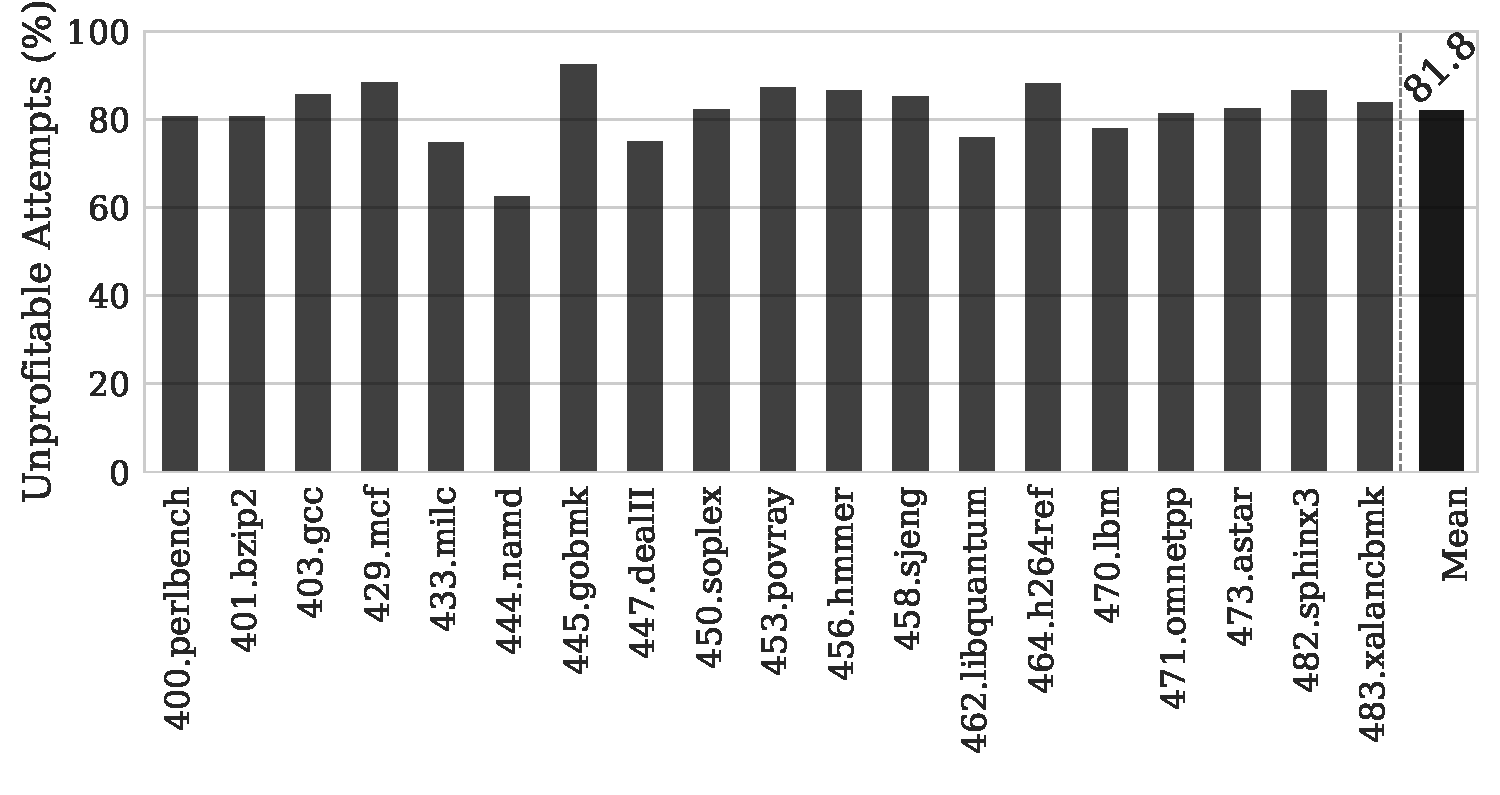
\includegraphics[width=0.5\textwidth]{figs/unprofitable-attempts.pdf}
  \vspace{-2.5em}
  \caption{An average of about 82\% of merging attempts are unprofitable.}
  \label{fig:unprofitable-attempts}
\end{figure}

%Figure~\ref{fig:compilation-breakdown} shows a breakdown of the time spent in different steps of the function merging optimization.
%As expected, this breakdown confirms that most of the compilation-time is spent merging functions, which includes both the sequence alignment and code generation.
%This also includes the time wasted producing unprofitable merged functions.
%Therefore, it is important to avoid merging unprofitable functions.

Figure~\ref{fig:unprofitable-compile-time-percentage} shows the time spent producing unprofitable merged functions relative to the total compilation time of the function merging optimization.
Since most of the merged functions are thrown away for being unprofitable, it is expected that most of the compilation time is also spent producing those merged functions.
However, this impact is also aggravated when several of the unprofitable merged functions are much larger than the profitable ones.

\begin{figure}[h]
  \centering
  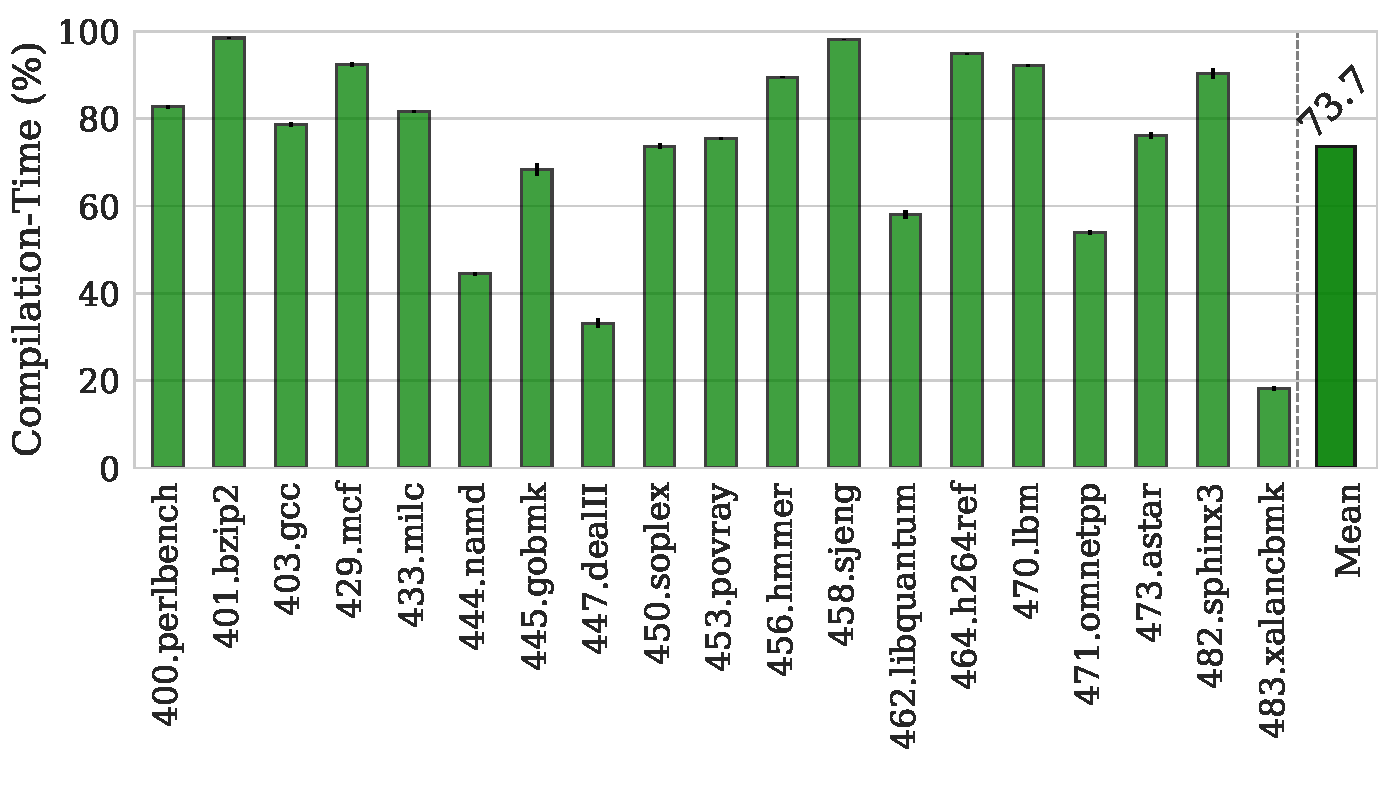
\includegraphics[width=0.5\textwidth]{figs/unprofitable-compile-time-percentage.pdf}
  \vspace{-2.5em}
  \caption{The percentage of compilation-time spent on unprofitable merge operations.}
  \label{fig:unprofitable-compile-time-percentage}
\end{figure}

Therefore, it is of utmost importance that we avoid merging unprofitable functions.
If we could eliminate all the time wasted on unprofitable merge operations, we would free compilation time for more useful computation.

In this paper, our goal is to develop a solution capable of identifying whether or not a given pair of functions can be profitably merged.
